\documentclass{article}\usepackage[]{graphicx}\usepackage[]{color}
% maxwidth is the original width if it is less than linewidth
% otherwise use linewidth (to make sure the graphics do not exceed the margin)
\makeatletter
\def\maxwidth{ %
  \ifdim\Gin@nat@width>\linewidth
    \linewidth
  \else
    \Gin@nat@width
  \fi
}
\makeatother

\definecolor{fgcolor}{rgb}{0.345, 0.345, 0.345}
\newcommand{\hlnum}[1]{\textcolor[rgb]{0.686,0.059,0.569}{#1}}%
\newcommand{\hlstr}[1]{\textcolor[rgb]{0.192,0.494,0.8}{#1}}%
\newcommand{\hlcom}[1]{\textcolor[rgb]{0.678,0.584,0.686}{\textit{#1}}}%
\newcommand{\hlopt}[1]{\textcolor[rgb]{0,0,0}{#1}}%
\newcommand{\hlstd}[1]{\textcolor[rgb]{0.345,0.345,0.345}{#1}}%
\newcommand{\hlkwa}[1]{\textcolor[rgb]{0.161,0.373,0.58}{\textbf{#1}}}%
\newcommand{\hlkwb}[1]{\textcolor[rgb]{0.69,0.353,0.396}{#1}}%
\newcommand{\hlkwc}[1]{\textcolor[rgb]{0.333,0.667,0.333}{#1}}%
\newcommand{\hlkwd}[1]{\textcolor[rgb]{0.737,0.353,0.396}{\textbf{#1}}}%
\let\hlipl\hlkwb

\usepackage{framed}
\makeatletter
\newenvironment{kframe}{%
 \def\at@end@of@kframe{}%
 \ifinner\ifhmode%
  \def\at@end@of@kframe{\end{minipage}}%
  \begin{minipage}{\columnwidth}%
 \fi\fi%
 \def\FrameCommand##1{\hskip\@totalleftmargin \hskip-\fboxsep
 \colorbox{shadecolor}{##1}\hskip-\fboxsep
     % There is no \\@totalrightmargin, so:
     \hskip-\linewidth \hskip-\@totalleftmargin \hskip\columnwidth}%
 \MakeFramed {\advance\hsize-\width
   \@totalleftmargin\z@ \linewidth\hsize
   \@setminipage}}%
 {\par\unskip\endMakeFramed%
 \at@end@of@kframe}
\makeatother

\definecolor{shadecolor}{rgb}{.97, .97, .97}
\definecolor{messagecolor}{rgb}{0, 0, 0}
\definecolor{warningcolor}{rgb}{1, 0, 1}
\definecolor{errorcolor}{rgb}{1, 0, 0}
\newenvironment{knitrout}{}{} % an empty environment to be redefined in TeX

\usepackage{alltt}[12pt]
\usepackage{Sweave}
\usepackage{float}
\usepackage{graphicx}
\usepackage{tabularx}
\usepackage{siunitx}
\usepackage{amssymb} % for math symbols
\usepackage{amsmath} % for aligning equations
\usepackage{mdframed}
\usepackage{natbib}
%\bibliographystyle{..//bib/styles/gcb}
\usepackage[hyphens]{url}
\usepackage[small]{caption}
\setlength{\captionmargin}{30pt}
\setlength{\abovecaptionskip}{0pt}
\setlength{\belowcaptionskip}{10pt}
\topmargin -1.5cm        
\oddsidemargin -0.04cm   
\evensidemargin -0.04cm
\textwidth 16.59cm
\textheight 21.94cm 
%\pagestyle{empty} %comment if want page numbers
\parskip 7.2pt
\renewcommand{\baselinestretch}{2}
\parindent 0pt
\usepackage{lineno}
\linenumbers
\usepackage{setspace}
\doublespacing

\newmdenv[
  topline=true,
  bottomline=true,
  skipabove=\topsep,
  skipbelow=\topsep
]{siderules}
\IfFileExists{upquote.sty}{\usepackage{upquote}}{}
\begin{document}

\renewcommand{\thetable}{\arabic{table}}
\renewcommand{\thefigure}{\arabic{figure}}
\renewcommand{\labelitemi}{$-$}

\renewcommand{\thesection}{\arabic{section}.}
\renewcommand\thesubsection{\arabic{section}.\arabic{subsection}} 

\begin{center}
\begin{tabular}{l c c c | c c c}
\cline{2-7}
& \multicolumn{3}{ c| }{1951-1983}
& \multicolumn{3}{ c }{1984-2016} \\ \cline{2-7}
& mean & 10\% & 90\% & mean & 10\% & 90\% \\
\hline
\textit{Aesculus hippocastanum} & 0.260 & 0.257 & 0.263 & 0.333 & 0.330 & 0.337  \\
\textit{Alnus glutinosa} & 0.265 & 0.261 & 0.268 & 0.352 & 0.348 & 0.357 \\
\textit{Betula pendula} & 0.265 & 0.263 & 0.268 & 0.353 & 0.349 & 0.356 \\
\textit{Fagus sylvatica} & 0.223 & 0.220 & 0.225 & 0.228 & 0.225 & 0.231 \\
\textit{Fraxinus excelsior} & 0.096 & 0.094 & 0.099 & 0.083 & 0.080 & 0.085 \\
\textit{Quercus robur} & 0.132 & 0.129 & 0.134 & 0.126 & 0.123 & 0.128 \\
\hline
\end{tabular}
\end{center}




{\begin{figure} [H]
  -\begin{center}
  -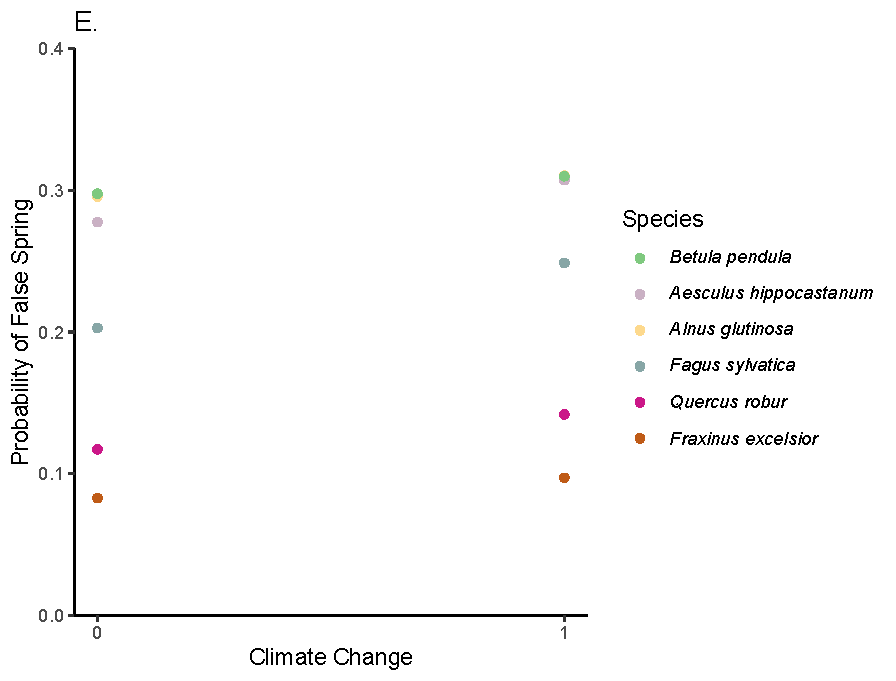
\includegraphics[width=12cm]{..//analyses/figures/InteractionPlots/ccxspecies_dots.pdf}
  -\caption{Marginal effects of climate change for each species}\label{fig:spp}
  -\end{center}
  -\end{figure}}
  
  {\begin{figure} [H]
  -\begin{center}
  -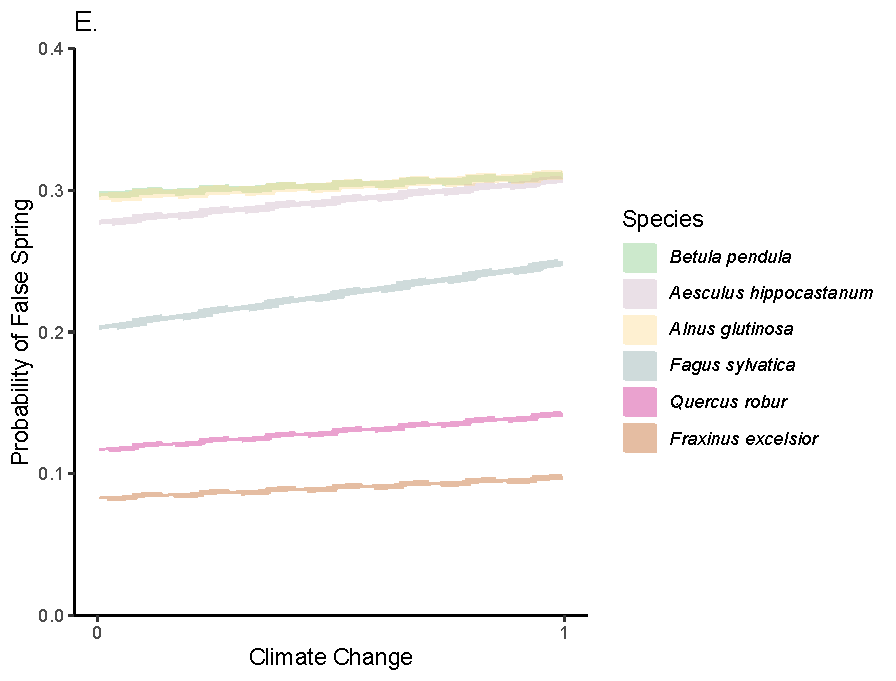
\includegraphics[width=12cm]{..//analyses/figures/InteractionPlots/ccxspecies_lines.pdf}
  -\caption{Marginal effects of climate change for each species}\label{fig:spp}
  -\end{center}
  -\end{figure}}


\end{document}
